\chapter{Detailní vzhled aplikace}
V~této části přílohy jsou znázorněny pohledy z~aktuální klientské aplikace, které by jinak rozrušovaly kontext práce.
Jako první obrazovka, která se uživateli ukáže je znázorněna na obrázku~\ref{fig:screen:index}.
Daná úvodní obrazovka by měla uživateli sdělit základní informace o~produktu apod.

Jestliže není uživatel autentizován, po kliknutí na dané tlačítko je přesměrován na stránku autentizační služby znázorněné na obrázku ~\ref{fig:screen:keycloak}.
V~opačném případě je uživatel již přesměrován na stránku aplikace, kde se zobrazí úvodní obrazovka ~\ref{fig:screen:home}.
Uživatel dále po rozkliknutí záložky \emph{My Homes} vidí všechny domácnosti, ve kterých je zařazen.(obrázek ~\ref{fig:screen:homes}).
A~poslední pohled z~aplikace pochází z~konkrétní místnosti, ve které je obsaženo jedno zařízení a lze ho tímto způsobem spravovat.(viz ~\ref{fig:screen:device})

\begin{figure}[hbt]
    \centering
    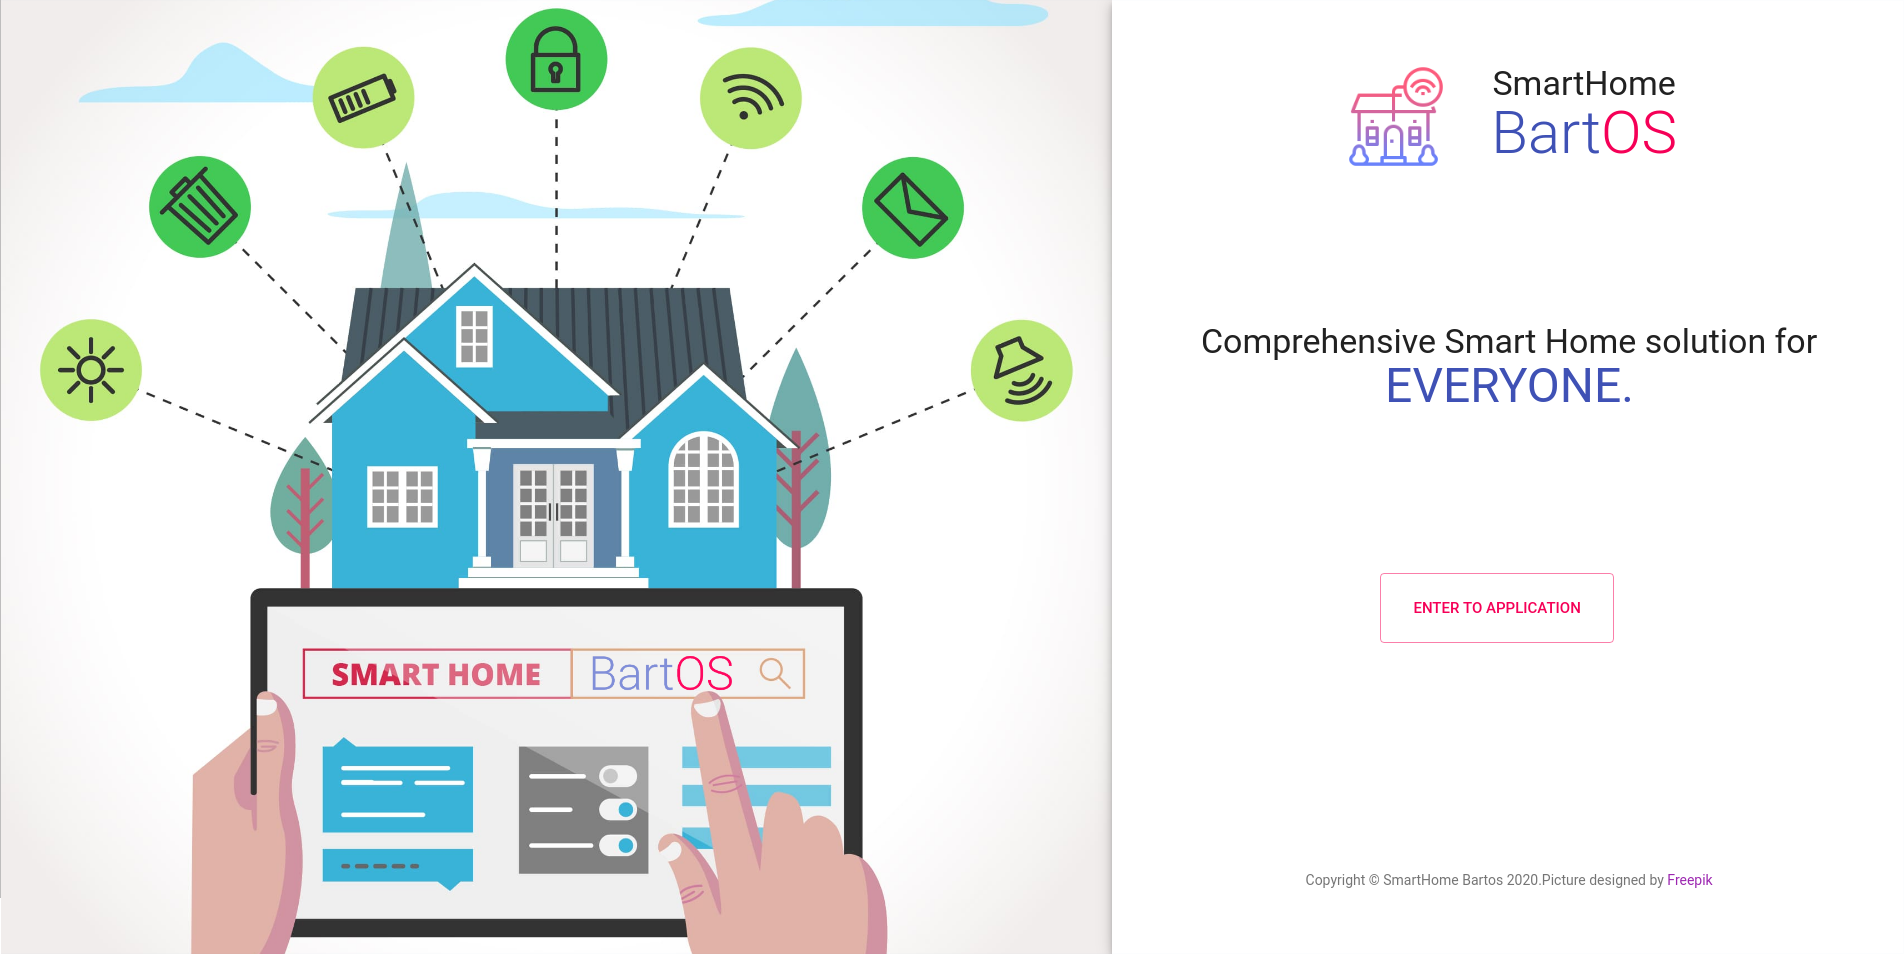
\includegraphics[width=1\linewidth]{obrazky-figures/screen/login.png}
    \caption{Úvodní obrazovka aplikace.}
    \label{fig:screen:index}
\end{figure}

\begin{figure}[hbt]
    \centering
    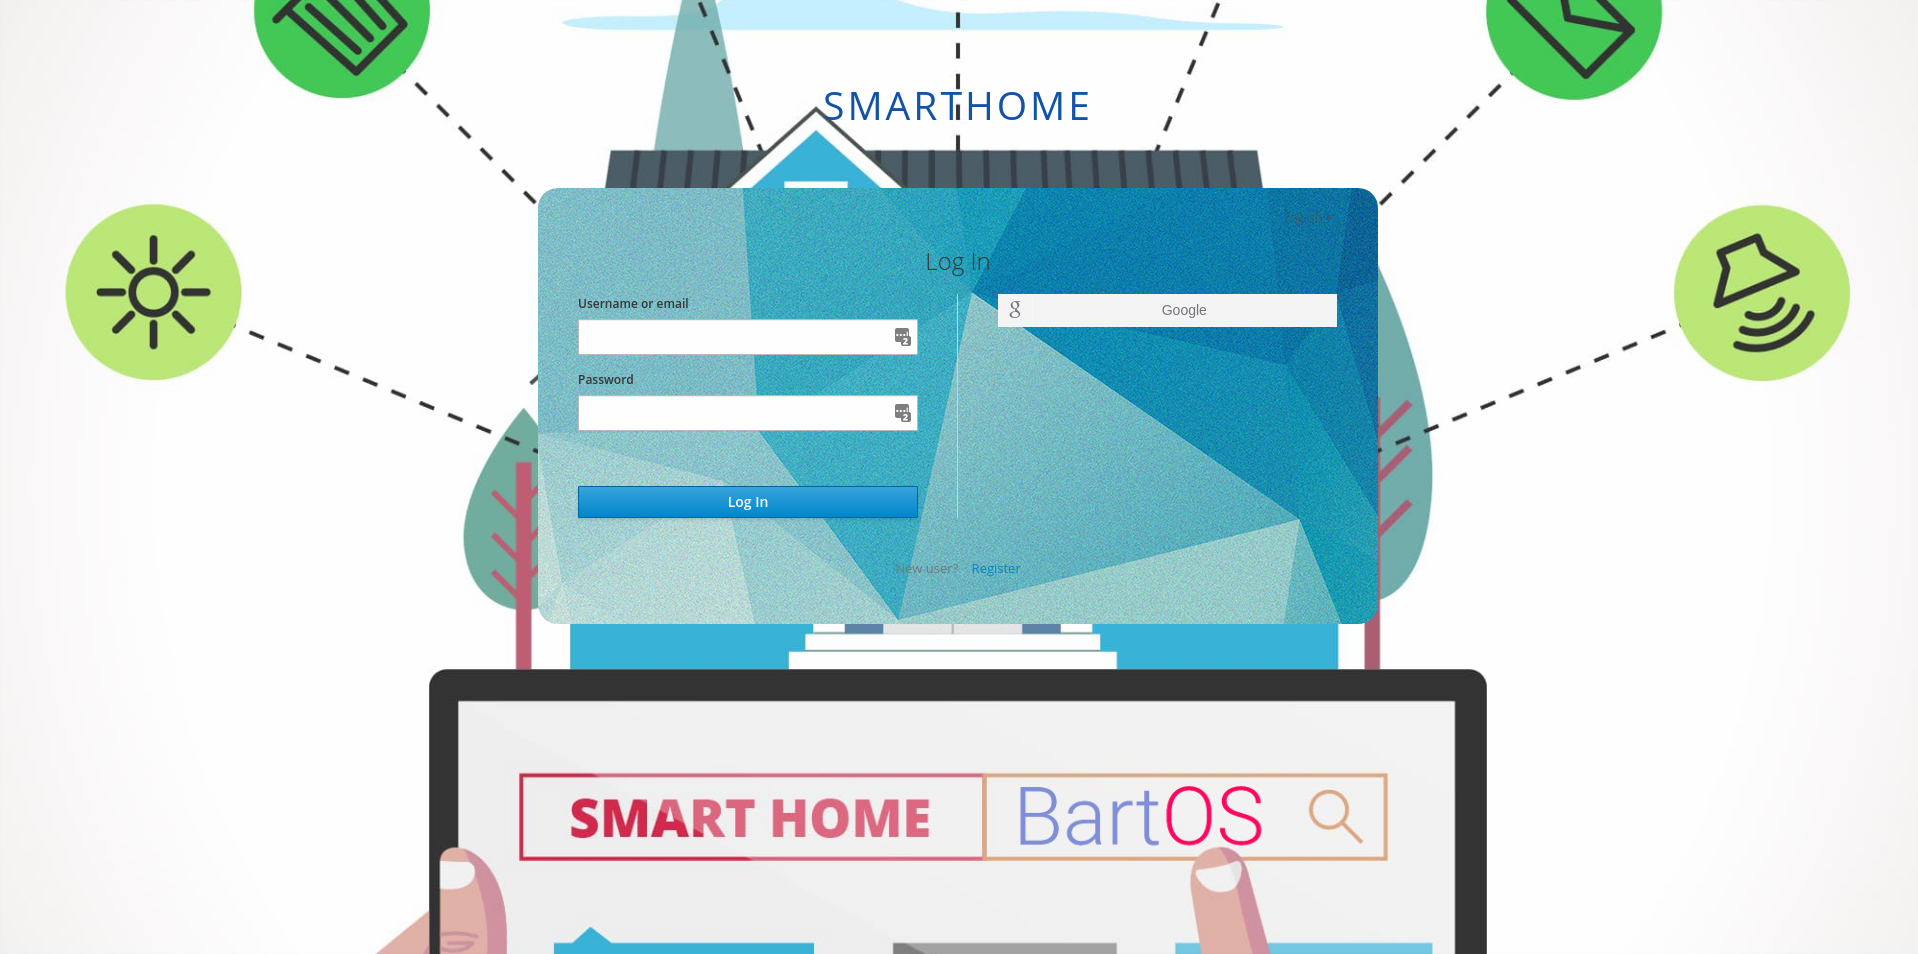
\includegraphics[width=1\linewidth]{obrazky-figures/screen/keycloak.png}
    \caption{Přihlašovací formulář u~autentizační služby.}
    \label{fig:screen:keycloak}
\end{figure}

\begin{figure}[hbt]
    \centering
    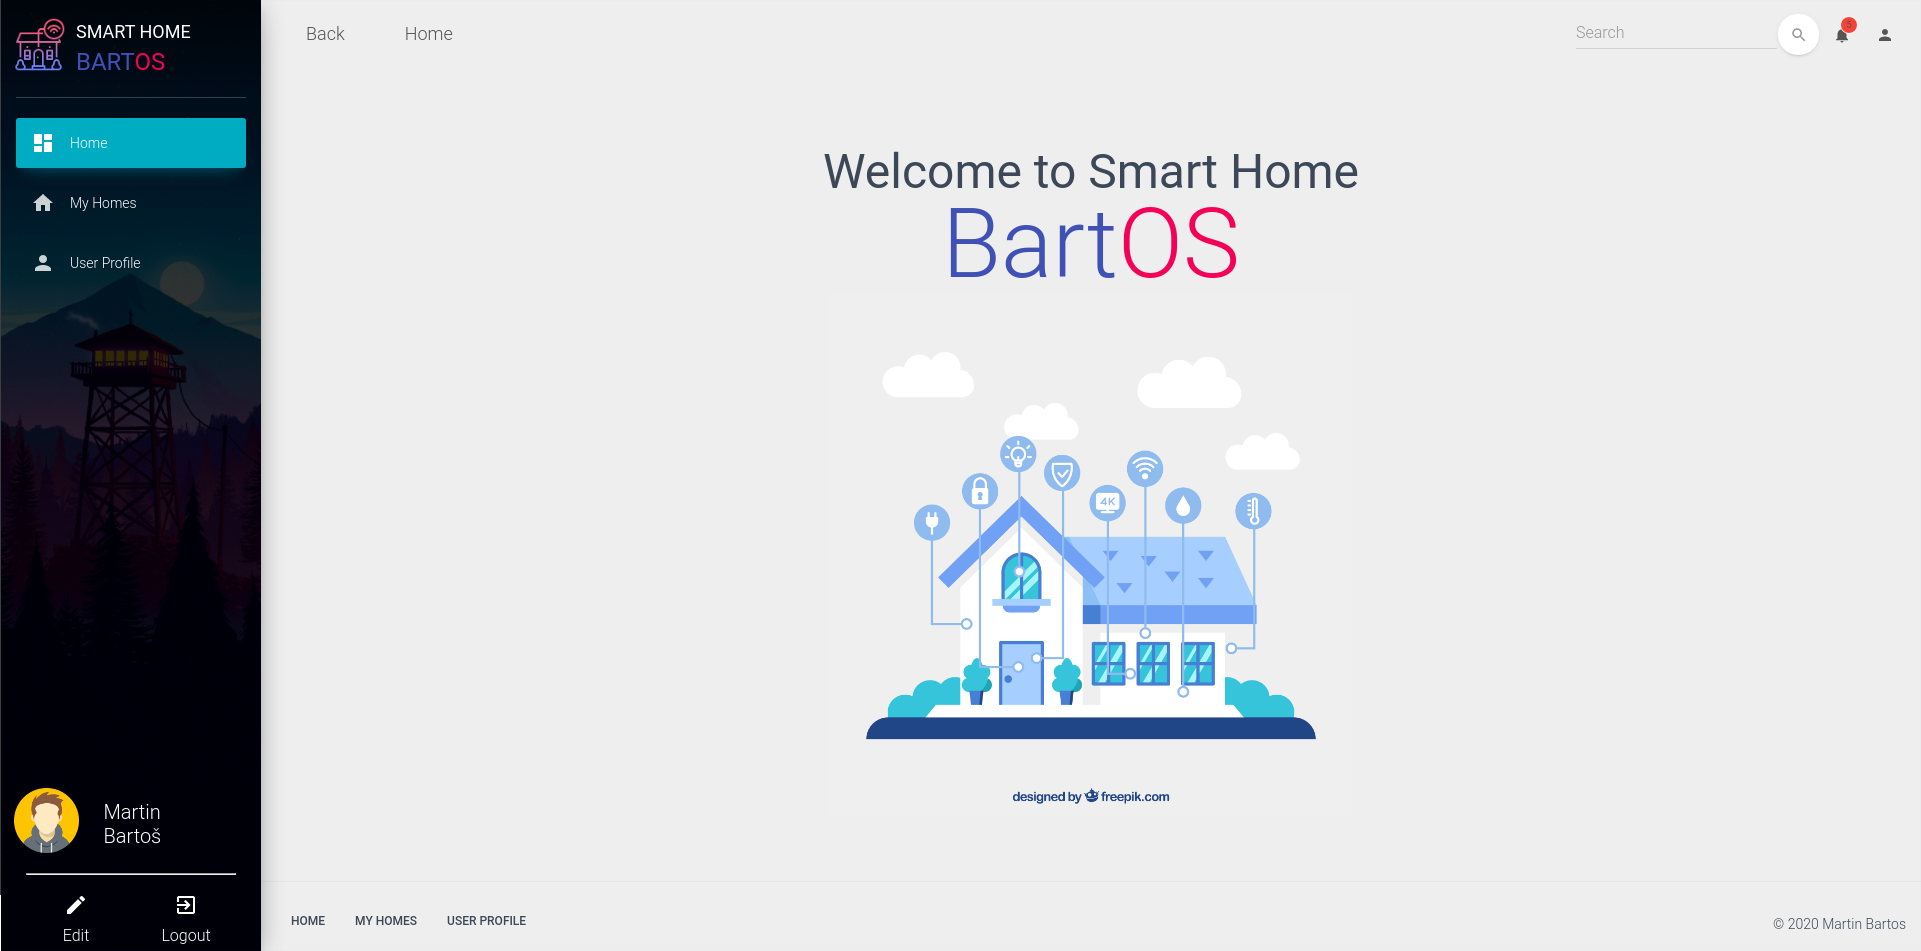
\includegraphics[width=1\linewidth]{obrazky-figures/screen/welcome.png}
    \caption{Uvítací obrazovka aplikace}
    \label{fig:screen:home}
\end{figure}

\begin{figure}[hbt]
    \centering
    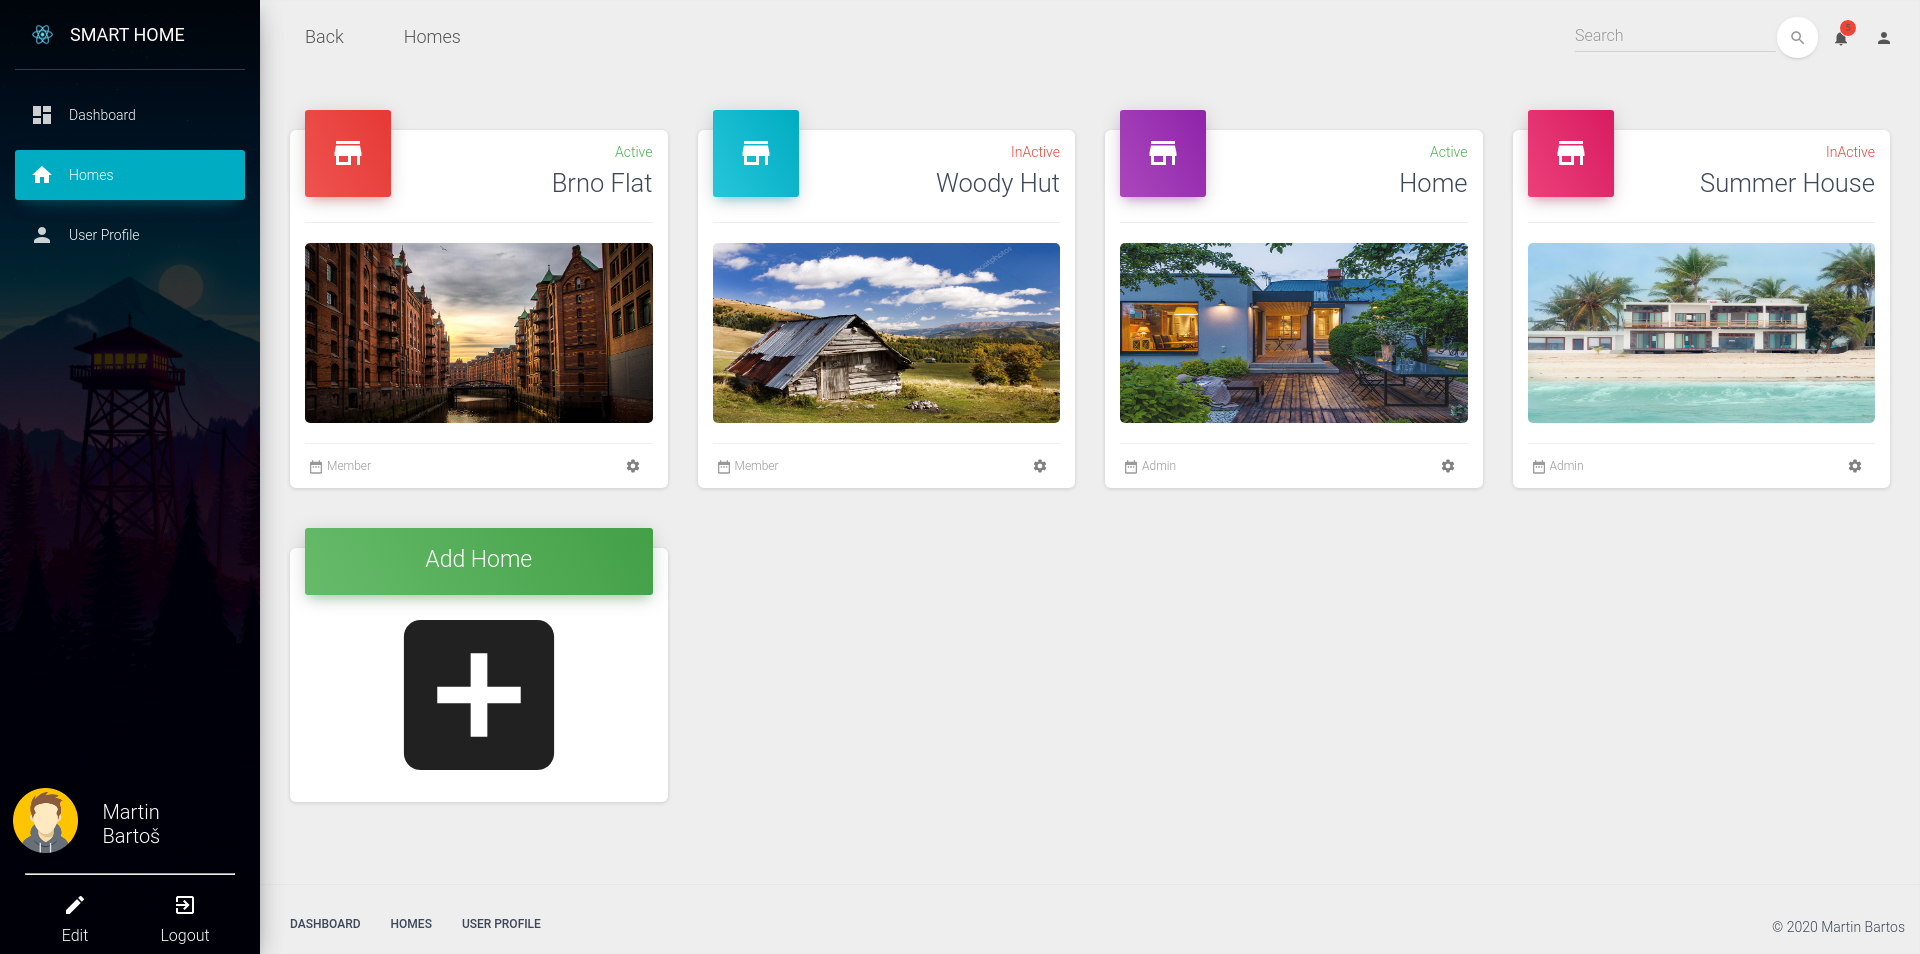
\includegraphics[width=1\linewidth]{obrazky-figures/actualView.png}
    \caption{Zobrazení všech domácností, ve kterých je uživatel obsažen.}
    \label{fig:screen:homes}
\end{figure}

\begin{figure}[hbt]
    \centering
    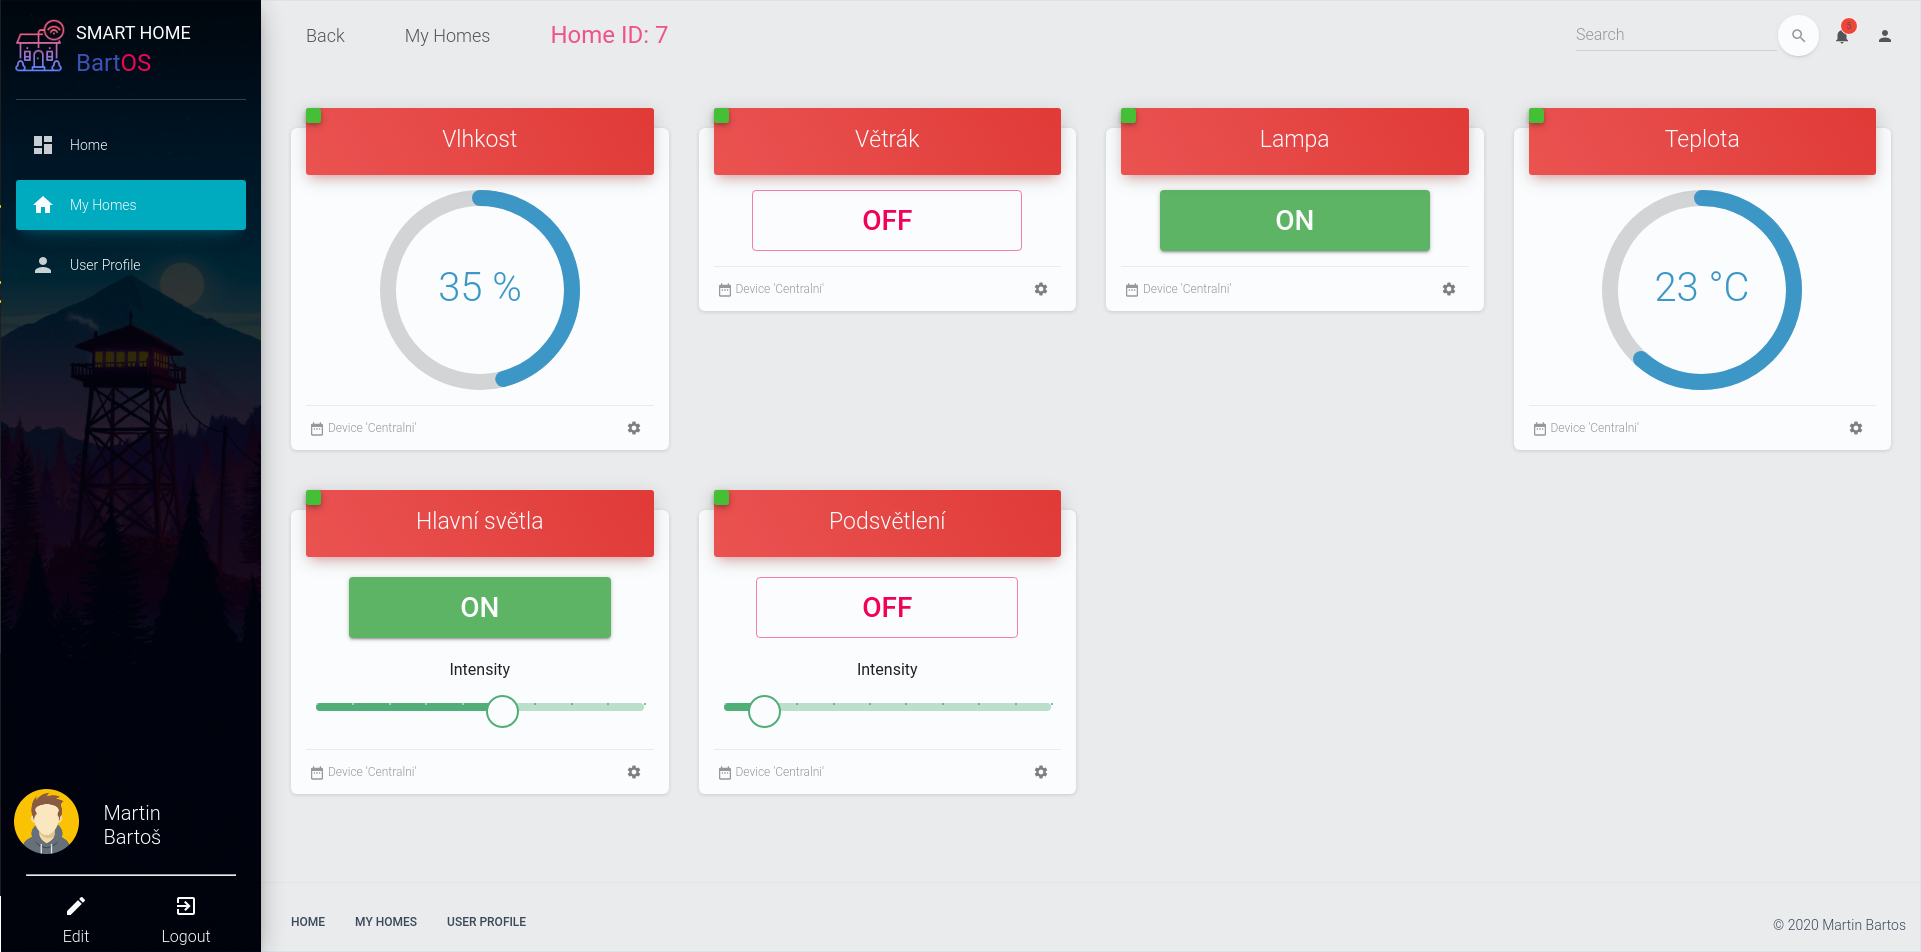
\includegraphics[width=1\linewidth]{obrazky-figures/screen/device.png}
    \caption{Ovládání zařízení v~určitém pokoji}
    \label{fig:screen:device}
\end{figure}

\chapter{Testovací zařízení}
V~této příloze lze nalézt testovací zařízení, která byla použita pro zkonstruování daného systému.
Vytvořeno bylo centrální zařízení, které slouží pro ovládání pokoje.
Zařízení dokáže, po připojení dalších periférií, měřit teplotu a vlhkost, ovládat sadu LED osvětlení a spínat 2 zařízení uzpůsobena na 230V.(např. větrák, topení)
Dále byly využity relé moduly dedikované pro mikrokontrolér \emph{ESP-01}.

Na obrázku~\ref{fig:dev:schematic} je znázorněné schéma zařízení potřebné pro výrobu DPS.
Většina je vyvedena externě z~desky pro případnou upravovatelnost schopnosti zařízení.
Na obrázku~\ref{fig:dev:dps} je vyobrazen návrh DPS, pomocí kterého byla deska zkonstruována.
Vyrobené testovací zařízení a 2 relé moduly jsou znázorněny na obrázku~\ref{fig:dev:actual}.

\begin{figure}[hbt]
    \centering
    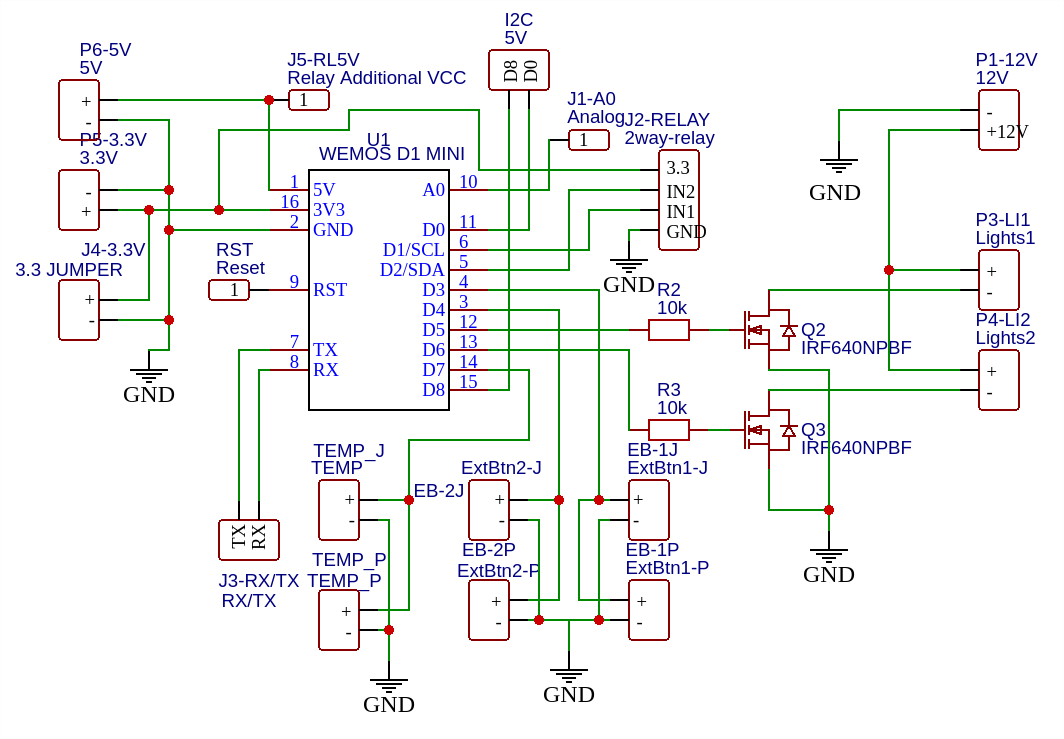
\includegraphics[width=1 \linewidth]{obrazky-figures/schematicNew.png}
    \caption{Návrh schématu centrálního zařízení}
    \label{fig:dev:schematic}
\end{figure}

\begin{figure}[hbt]
    \centering
    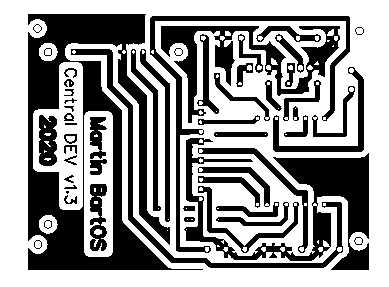
\includegraphics[width=0.7 \linewidth]{obrazky-figures/dps.png}
    \caption{Návrh DPS pro centrální zařízení}
    \label{fig:dev:dps}
\end{figure}

\begin{figure}[hbt]
    \centering
    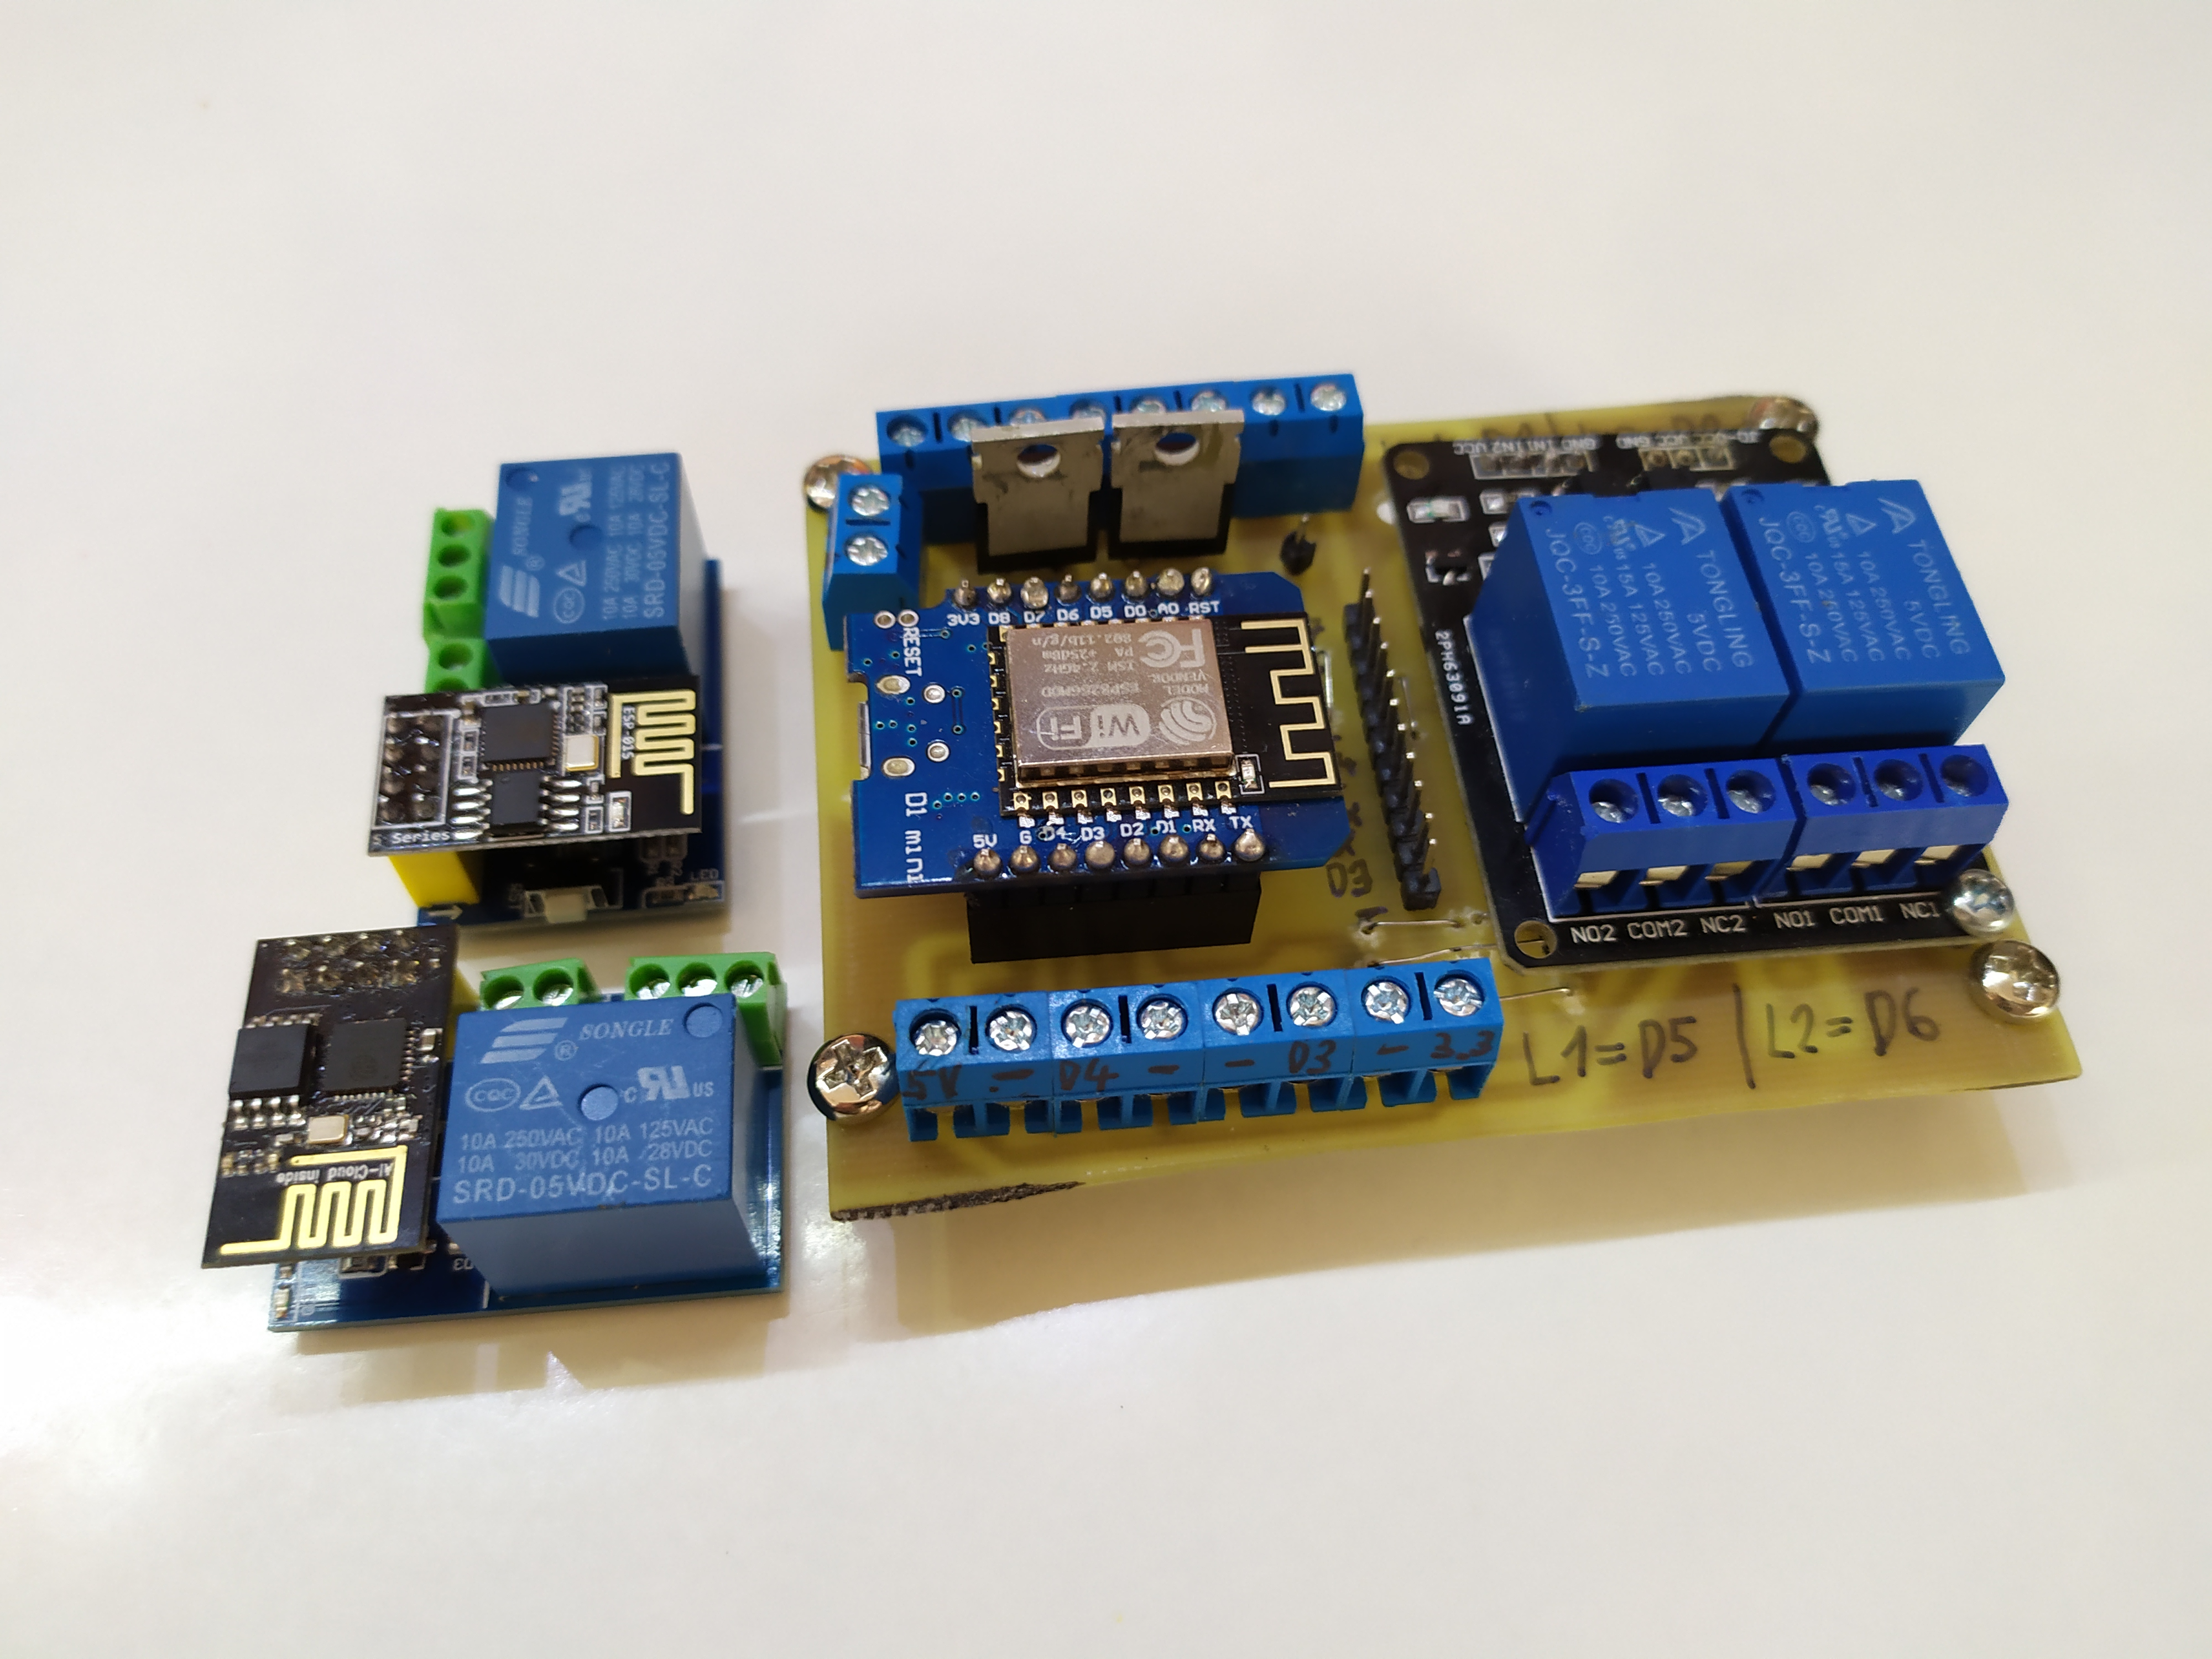
\includegraphics[width=0.9\linewidth]{obrazky-figures/testDevice.jpg}
    \caption{Vyrobené centrální zařízení a 2 relé moduly s~mikrokontrolérem \emph{ESP-01}.}
    \label{fig:dev:actual}
\end{figure}